\chapter{集合}\label{ch16}

\emph{We all behave like Maxwell’s demon. Organisms organize. In everyday experience lies the reason sober physicists across two centuries kept this cartoon fantasy alive. We sort the mail, build sand castles, solve jigsaw puzzles, separate wheat from chaff, rearrange chess pieces, collect stamps, alphabetize books, create symmetry, compose sonnets and sonatas, and put our rooms in order, and all this we do requires no great energy, as long as we can apply intelligence.}

\begin{flushright}
    ——James Gleick, The Information: A History, a Theory, a Flood
\end{flushright}

Rust标准库里包含几种\emph{集合(collection)},它们是在内存中存储数据的泛型类型。我们已经在本书的很多地方使用过集合,例如\texttt{Vec}和\texttt{HashMap}。在本章中,我们将详细介绍这两种类型的方法,以及其他六种标准集合。但在我们开始之前,让我们先讨论一下Rust的集合和其他语言中的集合的一些不同之处。

首先,移动和借用无处不在。Rust使用移动来避免深拷贝。这就是为什么\texttt{Vec<T>::push(item)}方法以值获取参数,而不是以引用。值会被移动进vector。\hyperref[ch04]{第4章}中的图展示了实践中的表现:在Rust中把一个\texttt{String}添加到\texttt{Vec<String>}中很快,因为Rust不需要拷贝字符串的字符数据,字符串的所有权归属也总是很清楚。

其次,当集合改变大小或者被修改的同时还有指向它们的数据的指针时,Rust不会有无效性错误——即悬垂指针。无效性错误是C++中另一种未定义行为的来源,即使在内存安全的语言中也可能导致\texttt{ConcurrentModificationException}。Rust借用检查器会在编译器检查出它们。

最后,Rust没有\texttt{null},因此我们将在其他语言中需要\texttt{null}的地方看到\texttt{Option}。

除了这些不同之外,Rust的集合可能正是你需要的。如果你是经验丰富的程序员并且时间不多,你可以跳过这部分,但不要跳过“\nameref{entry}”。

\section{概述}

\autoref{t16-1}展示了Rust的8种标准集合。它们都是泛型类型。

\begin{table}[htbp]
    \centering
    \caption{标准集合总结}
    \label{t16-1}
    \begin{tabular}{p{0.2\textwidth}p{0.2\textwidth}lll}
        \hline
        \multirow{2}{*}{\textbf{集合}}  & \multirow{2}{*}{\textbf{说明}} & \multicolumn{3}{l}{\textbf{其他语言中的类似集合类型}} \\
        \cline{3-5}
         & & \textbf{C++} & \textbf{Java} & \textbf{Python} \\
        \hline
        
        \texttt{Vec<T>} & 可增长的数组  & \texttt{vector} & \texttt{ArrayList} & \texttt{list}  \\
        \rowcolor{tablecolor}
        \texttt{VecDeque<T>} & 双端队列(可增长环形缓冲区) & \texttt{deque} & \texttt{ArrayDeque} & \texttt{collections.deque} \\
        \texttt{LinkedList<T>} & 双向链表 & \texttt{list} & \texttt{LinkedList} & —— \\
        \rowcolor{tablecolor}
        \texttt{BinaryHeap<T> where T: Ord} & 大顶堆 & \texttt{priority\_queue} & \texttt{PriorityQueue} & \texttt{heapq} \\
        \texttt{HashMap<K, V> where K: Eq + Hash} & 键值哈希表 & \texttt{unordered\_map} & \texttt{HashMap} & \texttt{dict} \\
        \rowcolor{tablecolor}
        \texttt{BTreeMap<K, V> where K: Ord} & 有序键值表 & \texttt{map} & \texttt{TreeMap} & —— \\
        \texttt{HashSet<T> where T: Eq + Hash} & 基于哈希的无序集合 & \texttt{unordered\_set} & \texttt{HashSet} & \texttt{set} \\
        \rowcolor{tablecolor}
        \texttt{BTreeSet<T> where T: Ord} & 有序集合 & \texttt{set} & \texttt{TreeSet} & —— \\
    \end{tabular}
\end{table}

\texttt{Vec<T>}、\texttt{HashMap<K, V>}、\texttt{HashSet<T>}是最常用的集合类型。其他的集合都有适用的场景。这一章将轮流讨论每一个集合类型:

\codeentry{Vec<T>}
\hangparagraph{一个客增唱的、在堆上分配的、\texttt{T}类值的数组。本章中大约一半的篇幅专门介绍\texttt{Vec}和它的有用的方法。}

\codeentry{VecDeque<T>}
\hangparagraph{类似于\texttt{Vec<T>},但是用作先进先出队列会更好。它支持高效地在首部和尾部添加或移除元素,但这种能力的代价是其他操作会稍微慢一点。}

\codeentry{BinaryHeap<T>}
\hangparagraph{一个优先队列。\texttt{BinaryHeap}中的值按照一定结构组织,因此总是可以高效地找到和移除最大值。}

\codeentry{HashMap<K, V>}
\hangparagraph{一个键值对的表。通过键查找值很快速。表中的条目以任意顺序存储。}

\codeentry{BTreeMap<K, V>}
\hangparagraph{类似于\texttt{HashMap<K, V>},但按键的顺序保持条目有序。一个\texttt{BTreeMap<String, i32>}按照\texttt{String}的比较顺序存储条目。除非你需要条目保持有序,否则\texttt{HashMap}会更快。}

\codeentry{HashSet<T>}
\hangparagraph{类型\texttt{T}的值的集合。添加和删除元素都很快,查询一个值是否在集合中也很快。}

\codeentry{BTreeSet<T>}
\hangparagraph{类似于\texttt{HashSet<T>},但保持元素有序。同样,除非你想要数据保持有序,否则\texttt{HashSet}会更快。}

因为\texttt{LinkedList}很少使用(并且在大多数情况下都有更好的替代,无论是性能还是接口),因此我们不会在这里介绍它。

\section{\texttt{Vec<T>}}

我们假设你对\texttt{Vec}已经有了一定了解,因为我们在本书的很多地方都已经使用过它。简要的介绍见“\nameref{vector}”。这里我们只会描述它的方法以及深入它的内部工作原理。

最简单的创建vector的方式是使用\texttt{vec!}宏:
\begin{minted}{Rust}
    // 创建一个空的vector
    let mut numbers: Vec<i32> = vec![];

    // 用给定的内容创建一个vector
    let words = vec!["step", "on", "no", "pets"];
    let mut buffer = vec![0u8; 1024];   // 1024个0字节
\end{minted}

正如我们在“\hyperref[ch04]{第4章}”所述,vector有三个字段:长度、容量、和一个指向堆上分配的缓冲区的指针。\autoref{f16-1}展示了上面的vector在内存中的视图。空vector,\texttt{numbers},初始长度为0。在它添加第一个元素之前不会有堆内存被分配。

\begin{figure}[htbp]
    \centering
    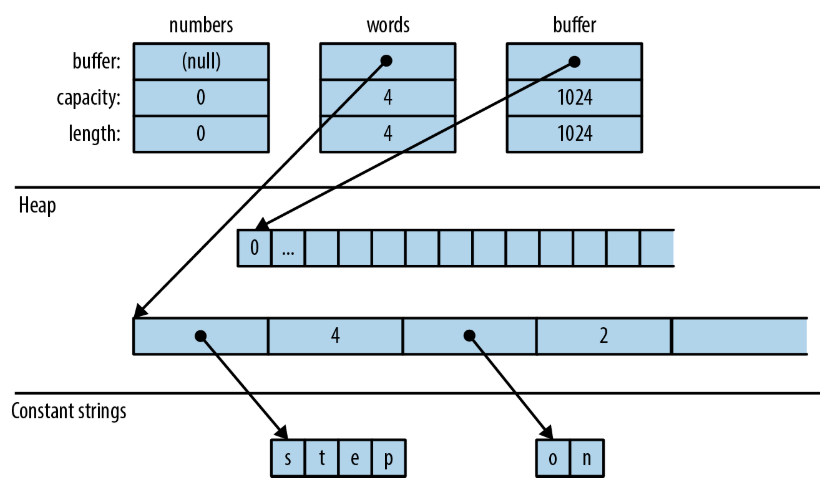
\includegraphics[width=0.9\textwidth]{../img/f16-1.png}
    \caption{vector的内存布局:words的每个元素是一个由指针和长度组成的\&str值}
    \label{f16-1}
\end{figure}

类似于所有集合,\texttt{Vec}实现了\texttt{std::iter::FromIterator},因此你可以对任何迭代器调用\texttt{.collect()}方法来创建一个vector,正如“\nameref{BuildColl}”中所述:
\begin{minted}{Rust}
    // 将一个其他集合转换成vector
    let my_vec = my_set.into_iter().collect::<Vec<String>>();
\end{minted}

\subsection{访问元素}
通过索引访问数组、切片或vector的元素非常直观:
\begin{minted}{Rust}
    // 获取一个元素的引用
    let first_line = &lines[0];

    // 获取一个元素的拷贝 
    let fifth_number = numbers[4];          // 需要Copy
    let second_number = lines[1].clone();   // 需要Clone

    // 获取一个切片的引用
    let my_ref = &buffer[4..12];

    // 获取一个切片的拷贝
    let my_copy = buffer[4..12].to_vec();   // 需要Clone
\end{minted}

当索引越界时所有这些方式都会panic。

Rust对数字类型很挑剔,vector也不例外。vector的长度和索引都是\texttt{usize}类型。尝试使用\texttt{u32}、\texttt{u64}、\texttt{isize}作为vector的索引会导致错误。必要时你可以使用\texttt{n as usize}来转换,见“\nameref{cast}”。

有几种方法提供了便捷地访问vector或切片的特定元素的方法(注意所有的切片方法都能用于数组和vector):
\codeentry{slice.first()}
\hangparagraph{返回\texttt{slice}的第一个元素的引用。返回类型是\texttt{Option<\&T>},因此如果\texttt{slice}为空时返回值为\texttt{None},不为空时返回值为\texttt{Some(\&slice[0])}}:
\begin{minted}{Rust}
    if let Some(item) = v.first() {
        println!("We got one! {}", item);
    }
\end{minted}

\codeentry{slice.last()}
\hangparagraph{和上边相似,不过返回最有一个元素的引用。}

\codeentry{slice.get(index)}
\hangparagraph{返回\texttt{slice[index]}的引用,如果存在的话。如果\texttt{slice}的元素数量小于\texttt{index+1},那么返回\texttt{None}}:
\begin{minted}{Rust}
    let slice = [0, 1, 2, 3];
    assert_eq!(slice.get(2), Some(&2));
    assert_eq!(slice.get(4), None);
\end{minted}

\codeentry{slice.first\_mut(), slice.last\_mut(), slice.get\_mut(index)}
\hangparagraph{与上面的类似,不过借用\texttt{mut}引用:}
\begin{minted}{Rust}
    let mut slice = [0, 1, 2, 3];
    {
        let last = slice.last_mut().unwrap();   // 最后一个元素类型:&mut i32
        assert_eq!(*last, 3);
        *last = 100;
    }
\end{minted}

因为以值返回\texttt{T}意味着移动它,因此访问元素的方法通常返回元素的引用。

一个例外是\texttt{.to\_vec()}方法,它获取拷贝:

\codeentry{slice.to\_vec()}
\hangparagraph{克隆整个切片,返回一个新的vector:}
\begin{minted}{Rust}
    let v = [1, 2, 3, 4, 5, 6, 7, 8, 9];
    assert_eq!(v.to_vec(),
               vec![1, 2, 3, 4, 5, 6, 7, 8, 9]);
    assert_eq!(v[0..6].to_vec(),
               vec![1, 2, 3, 4, 5, 6]);
\end{minted}
\hangparagraph{只有当元素可以拷贝时这个方法才可用,即\texttt{where T: Clone}}

\subsection{迭代}\label{Iteration}
vector和切片可以以值或者以引用迭代,遵循“\nameref{IntoIter}”中介绍的模式:
\begin{itemize}
    \item 迭代\texttt{Vec<T>}会产生\texttt{T}类型的item。元素被逐个移出vector消耗掉。
    \item 迭代\texttt{\&[T; N], \&[T], \&Vec<T>}——即数组、切片或vector的引用——会产生\texttt{\&T}类型的item,每一个item指向一个元素,不会移动元素。
    \item 迭代\texttt{\&mut [T; N], \&mut [T], \&mut Vec<T>}产生\texttt{\&mut T}类型的item。
\end{itemize}

数组、切片和vector还有\texttt{.iter()}和\texttt{.iter\_mut()}方法(见“\nameref{IterMethod}”)创建产生元素的引用的迭代器。

我们将在“\nameref{split}”中介绍一些更有趣的迭代切片的方法。

\subsection{增长和缩减vector}
数组、切片或vector的\emph{长度(length)}是它包含的元素的数量:

\codeentry{slice.len()}
\hangparagraph{返回一个\texttt{slice}的长度,类型为\texttt{usize}。}

\codeentry{slice.is\_empty()}
\hangparagraph{当\texttt{slice}不包含元素时为真(即\texttt{slice.len() == 0})。}

本节剩余的方法都是关于增长和缩减vector。它们不能用于数组和切片,因为它们一旦被创建之后就不能改变大小。

vector的所有元素都存储在一个在堆上分配的连续内存块中。vector的\emph{容量(capacity)}是指当前的内存块中最多能存储的元素数量。\texttt{Vec}通常会替你管理容量,当需要增长时它会自动分配更大的缓冲区并把元素都移动过去。还有一些显式管理容量的方法:

\codeentry{Vec::with\_capacity(n)}
\hangparagraph{创建一个容量为\texttt{n}的新的空vector。}

\codeentry{vec.capacity()}
\hangparagraph{返回\texttt{vec}的容量,类型是\texttt{usize}。\texttt{vec.capacity() >= vec.len()}总是为真。}

\codeentry{vec.reserve(n)}
\hangparagraph{保证vector的剩余空间至少还能再存储\texttt{n}个或更多元素:即\texttt{vec.capacity()}至少是\texttt{vec.len() + n}。如果已经有足够的空间,它不做任何事。否则,它会分配一个更大的缓冲区并且把vector的内容移动过去。}

\codeentry{vec.reserve\_exact(n)}
\hangparagraph{类似于\texttt{vec.reserve(n)},但告诉\texttt{vec}不要为未来的增长分配额外的空间。调用它之后,\texttt{vec.capacity()}等于\texttt{vec.len() + n}。}

\codeentry{vec.shrink\_to\_fit()}
\hangparagraph{当\texttt{vec.capacity()}大于\texttt{vec.len()}时尝试释放额外的内存。}

\texttt{Vec<T>}有很多添加或移除元素的方法,同时改变vector的长度。所有这些方法都以\texttt{mut}引用获取\texttt{self}参数。

下面这两个方法在vector的末尾添加或移除一个元素:

\codeentry{vec.push(value)}
\hangparagraph{把\texttt{value}添加到\texttt{vec}的末尾。}

\codeentry{vec.pop()}
\hangparagraph{移除并返回最后一个元素。返回类型是\texttt{Option<T>}。当vector已经为空时返回\texttt{None},否则返回\texttt{Some(x)}。}

注意\texttt{.push()}以值而不是以引用获取参数。类似的,\texttt{.pop()}返回被弹出的值,而不是引用。本节中剩余的大部分方法也是这样。它们从vector移出或移进值。

这两个方法向vector中添加值或者从vector中移出值:
\codeentry{vec.insert(index, value)}
\hangparagraph{在\texttt{vec[index]}处插入给定的\texttt{value},把\texttt{vec[index..]}中的值都向后移动一个位置来腾出空间。如果\texttt{index > vec.len()}会panic。}

\codeentry{vec.remove(index)}
\hangparagraph{移除并返回\texttt{vec[index]},把\texttt{vec[index+1..]}中的值向左移动一个位置来消除缝隙。}

\texttt{.insert()}和\texttt{.remove()}都很慢,因为有很多元素需要移动。

有四个方法可以将vector的长度调整为指定值:

\codeentry{vec.resize(new\_len, value)}
\hangparagraph{将\texttt{vec}的长度设为\texttt{new\_len}。如果这会增大\texttt{vec}的长度,将会用\texttt{value}的拷贝填充新空间。元素的类型必须实现了\texttt{Clone} trait。}

\codeentry{vec.resize\_with(new\_len, closure)}
\hangparagraph{类似于\texttt{vec.resize},但调用闭包来构造每一个新元素。它可以用于元素没有实现\texttt{Clone}的vector。}

\codeentry{vec.truncate(new\_len)}
\hangparagraph{将\texttt{vec}的长度缩减到\texttt{new\_len},丢弃\texttt{vec[new\_len..]}范围内的所有元素。如果\texttt{vec.len()}小于等于\texttt{new\_len},那么什么也不做。}

\codeentry{vec.clear()}
\hangparagraph{删除\texttt{vec}的所有元素。等价于\texttt{vec.truncate(0)}。}

有四个方法可以一次添加或移除很多元素:

\codeentry{vec.extend(iterable)}
\hangparagraph{将\texttt{iterable}的所有item按顺序添加到\texttt{vec}的末尾。它类似于多值版本的\texttt{.push()}。\texttt{iterable}参数可以是任何实现了\texttt{IntoIterator<Item=T>}。}
\hangparagraph{这个方法如此有用以至于有一个专门的trait \texttt{Extend},所有的标准集合都实现了它。不幸的是,这导致\texttt{rustdoc}将\texttt{.extend()}和其他trait的方法放在生成的HTML底部的一堆方法中,因此当你需要它时很难找到它。你必须记住它!更多内容见“\nameref{extend}”。}

\codeentry{vec.split\_off(index)}
\hangparagraph{类似于\texttt{vec.truncate(index)},除了它返回一个\texttt{Vec<T>}包含\texttt{vec}尾部被移除的元素。它类似于\texttt{.pop()}的多值版本。}

\codeentry{vec.append(\&mut vec2)}
\hangparagraph{这会把\texttt{vec2}的所有元素移动进\texttt{vec},其中\texttt{vec2}是另一个\texttt{Vec<T>}类型的vector。调用之后,\texttt{vec2}变为空。}
\hangparagraph{这类似于\texttt{vec.extend(vec2)},除了调用之后\texttt{vec2}仍然存在,并且容量不变。}

\codeentry{vec.drain(range)}
\hangparagraph{这会从\texttt{vec}中移除范围\texttt{vec[range]},并返回一个迭代被移除元素的迭代器,其中\texttt{range}是一个范围值,例如\texttt{..}或\texttt{0..4}。}

还有一些选择性移除vector元素的古怪方法:
\codeentry{vec.retain(test)}
\hangparagraph{移除所有没有通过给定测试的方法。\texttt{test}参数是一个实现了\texttt{FnMut(\&T) -> bool}的函数或闭包。对于\texttt{vec}的每一个元素,它会调用\texttt{test(\&element)},如果返回\texttt{false},元素将会被移出vector然后丢弃。}
\hangparagraph{不考虑性能的话,这类似于:}
\begin{minted}{Rust}
    vec = vec.into_iter().filter(test).collect();
\end{minted}

\codeentry{vec.dedup()}
\hangparagraph{丢弃相邻的重复元素。它类似于Unix的\texttt{uniq} shell工具。它会扫描\texttt{vec}中寻找相邻的重复元素,然后丢弃掉多余的重复值,只留下一个:}
\begin{minted}{Rust}
    let mut byte_vec = b"Missssssissippi".to_vec();
    byte_vec.dedup();
    assert_eq!(&byte_vec, b"Misisipi");
\end{minted}
\hangparagraph{注意最后的输出中仍然有两个\texttt{'s'}字符。这个方法只移除\emph{相邻的(adjacent)}重复值。为了移除所有的重复值,你有三种选择:调用\texttt{.dedup()}之前先排序vector,将数据移动到一个“\nameref{set}”,或者(为了保持元素原本的顺序)使用这个\texttt{.retain()}技巧:}
\begin{minted}{Rust}
    let mut byte_vec = b"Missssssissippi".to_vec();

    let mut seen = HashSet::new();
    byte_vec.retain(|r| seen.insert(*r));

    assert_eq!(&byte_vec, b"Misp");
\end{minted}
\hangparagraph{这段代码的原理是当集合中已经包含要插入的item时\texttt{.insert()}会返回\texttt{false}。}

\codeentry{vec.dedup\_by(same)}
\hangparagraph{类似于\texttt{vec.dedup()},但它使用函数或者闭包\texttt{same(\&mut elem1, \&mut elem2)},而不是\texttt{==}运算符,来检查两个相邻元素是否被认为相等。}

\codeentry{vec.dedup\_by\_key(key)}
\hangparagraph{类似于\texttt{vec.dedup()},但当\texttt{key(\&mut elem1) == key(\&mut elem2)}时它认为两个元素相等。}
\hangparagraph{例如,如果\texttt{errors}是一个\texttt{Vec<Box<dyn Error>>},你可以写:}
\begin{minted}{Rust}
    // 移除消息重复的错误。
    errors.dedup_by_key(|err| err.to_string());
\end{minted}

这一节介绍的所有方法中,只有\texttt{.resize()}可能会拷贝值。其他的通过移动值来工作。

\subsection{连接}
两个方法可以用于\emph{数组的数组(array of array)},即元素类型是数组、切片、vector的数组、切片、vector:

\codeentry{slices.concat()}
\hangparagraph{返回一个所有切片连接成的vector:}
\begin{minted}{Rust}
    assert_eq!([[1, 2], [3, 4], [5, 6]].concat(),
               vec![1, 2, 3, 4, 5, 6]);
\end{minted}

\codeentry{slices.join(\&separator)}
\hangparagraph{同上,除了会在切片之间插入\texttt{separator}的拷贝:}
\begin{minted}{Rust}
    assert_eq!([[1, 2], [3, 4], [5, 6]].join(&0),
               vec![1, 2, 0, 3, 4, 0, 5, 6]);
\end{minted}

\subsection{切分}\label{split}
很容易一次获得数组、切片、vector中的很多元素的非\texttt{mut}引用:
\begin{minted}{Rust}
    let v = vec![0, 1, 2, 3];
    let a = &v[i];
    let b = &v[j];

    let mid = v.len() / 2;
    let front_half = &v[..mid];
    let back_half = &v[mid..];
\end{minted}

但一次获得多个\texttt{mut}引用不是这么容易:
\begin{minted}{Rust}
    let mut v = vec![0, 1, 2, 3];
    let a = &mut v[i];
    let b = &mut v[j];  // error: 不能同时借用`v`的
                        // 多个可变引用。

    *a = 6;             // 引用`a`和`b`在这里使用了,
    *b = 7;             // 因此它们的生命周期一定会重叠。
\end{minted}

Rust禁止这样,因为如果\texttt{i == j},那么\texttt{a}和\texttt{b}将是同一个整数的两个\texttt{mut}引用,这违背了Rust的安全性的规则。(见“\nameref{ShareVSMut}”)。

Rust有几个方法可以一次借用数组、切片、vector的两个或更多元素的\texttt{mut}引用。和上面的代码不同,这些方法是安全的,因为它们从设计上保证了只会把数组分割成\emph{非重叠(nonoverlapping)区域}。这些方法也可以用于非\texttt{mut}切片,因此它们有\texttt{mut}和非\texttt{mut}版本。

\begin{figure}[htbp]
    \centering
    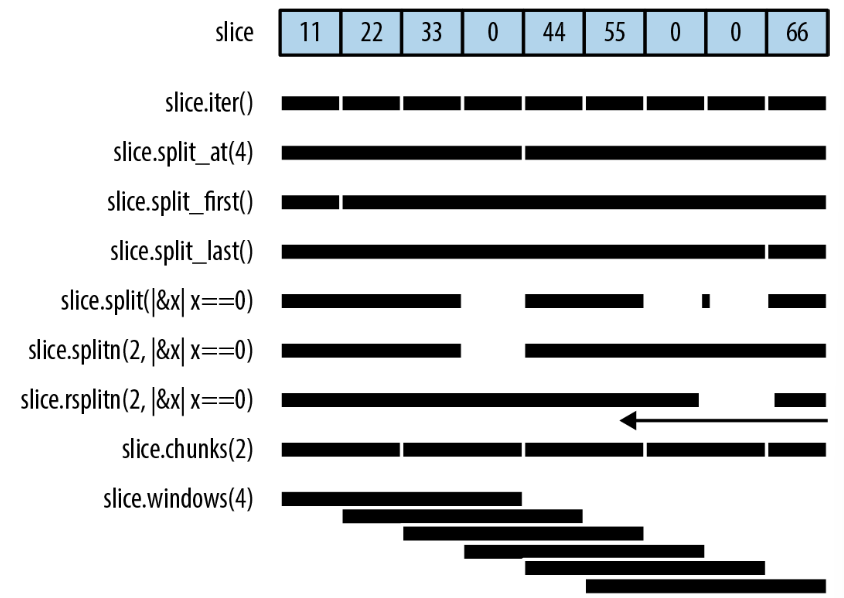
\includegraphics[width=0.9\textwidth]{../img/f16-2.png}
    \caption{分隔方法展示(注意:\texttt{slice.split()}输出中的小矩形是空的切片,因为两侧都是分隔符,\texttt{rsplitn}的输出是按照从后往前的顺序,这一点和其他的不同。}
    \label{f16-2}
\end{figure}

这些方法中没有一个会直接修改数组、切片或vector;它们都返回部分数据的引用:
\codeentry{slice.iter(), slice.iter\_mut()}
\hangparagraph{产生\texttt{slice}的每个元素的引用。我们在“\nameref{Iteration}”中已经介绍过它们。}

\codeentry{slice.split\_at(index), slice.split\_at\_mut(index)}
\hangparagraph{将一个切片划分为两个,返回一个pair。\texttt{slice.split\_at(index)}等价于\texttt{(\&slice[..index], \&slice[index..])}。如果\texttt{index}越界会panic。}

\codeentry{slice.split\_first(), slice.split\_first\_mut()}
\hangparagraph{也返回一个pair:第一个元素的引用(\texttt{slice[0]})和其余所有元素的切片引用(\texttt{slice[1..]})。}
\hangparagraph{\texttt{.spilt\_first()}的返回值类型是\texttt{Option<(\&T, \&[T])>};如果\texttt{slice}为空,返回\texttt{None}。}

\codeentry{slice.split\_last(), slice.split\_last\_mut()}
\hangparagraph{类似上一个,不过划分出最后一个元素而不是第一个。}
\hangparagraph{\texttt{.split\_last()}的返回类型是\texttt{Option<(\&T, \&[T])>}。}

\codeentry{slice.split(is\_sep), slice.split\_mut(is\_sep)}
\hangparagraph{将\texttt{slice}切分成一个或更多子切片,使用函数或闭包\texttt{is\_sep}来判断在哪里切分。它们返回一个迭代子切片的迭代器。}
\hangparagraph{当你消耗迭代器时,它会对切片中的每个元素调用\texttt{is\_sep(\&element)}。如果\texttt{is\_sep(\&element)}返回\texttt{true},那么这个元素就是一个分隔符。分隔符不包含在任何输出的字切片中。}
\hangparagraph{输出总是包含至少一个子切片,每有一个分隔符就加一个子切片。如果有相邻的分隔符或者\texttt{slice}的两端是分隔符都会产生空的子切片。}

\codeentry{slice.rsplit(is\_sep), slice.rsplit\_mut(is\_sep)}
\hangparagraph{类似于\texttt{slice}和\texttt{slice\_mut},但从最后一个切片开始。}

\codeentry{slice.splitn(n, is\_sep), slice.splitn\_mut(n, is\_sep)}
\hangparagraph{类似上面的方法,不过最多产生\texttt{n}个子切片。当发现了前\texttt{n-1}个切片之后就不会再调用\texttt{is\_sep}。最后一个字切片将包含剩余的所有元素。}

\codeentry{slice.rsplitn(n, is\_sep), slice.rsplitn\_mut(n, is\_sep)}
\hangparagraph{类似于\texttt{.splitn()}和\texttt{.splitn\_mut()},除了反向扫描切片。就是说,这个方法会在切片中\emph{最后}\texttt{n-1}个分隔符处切分,而不是前\texttt{n-1}个,并且从尾部开始产生子切片。}

\codeentry{slice.chunks(n), slice.chunks\_mut(n)}
\hangparagraph{返回一个产生长度为\texttt{n}的非重叠子切片的迭代器。如果\texttt{n}不能整除\texttt{slice.len()},最后一个块的元素数量将小于\texttt{n}。}

\codeentry{slice.rchunks(n), slick.rchunks\_mut(n)}
\hangparagraph{类似于\texttt{slice.chunks()}和\texttt{slice.chunks\_mut()},但是从切片的尾部开始。}

\codeentry{slice.chunks\_exact(n), slice.chunks\_exact\_mut(n)}
\hangparagraph{返回一个产生长度为\texttt{n}的非重叠子切片的迭代器。如果\texttt{n}不能整除\texttt{slice.len()},最后一个块(元素数量小于\texttt{n})可以通过结果的\texttt{remainder()}方法获得。}

\codeentry{slice.rchunks\_exact(n), slice.rchunks\_exact\_mut(n)}
\hangparagraph{类似于\texttt{slice.chunks\_exact}和\texttt{slice.chunks\_exact\_mut},但从切片的尾部开始。}

还有一些其他迭代子切片的方法:
\codeentry{slice.windows(n)}
\hangparagraph{返回一个效果类似于“滑动窗口”的迭代器。它产生\texttt{slice}中相邻的\texttt{n}个元素的子切片。第一个产生的值是\texttt{\&slice[0..n]},第二个是\texttt{\&slice[1..n+1]},以此类推。}
\hangparagraph{如果\texttt{n}大于\texttt{slice}的长度,将不会产生切片。如果\texttt{n}是0,这个方法会panic。}
\hangparagraph{例如,如果\texttt{days.len() == 31},那么我们可以调用\texttt{days.windows(7)}产生\texttt{days}中所有7天的区间。}
\hangparagraph{在探索数据列的变化趋势时一个大小为2的滑动窗口会很有用:}
\begin{minted}{Rust}
    let changes = daily_high\_temperatures
                      .windows(2)           // 获得相邻天的温度
                      .map(|w| w[1] - w[0]) // 温度改变了多少
                      .collect::<Vec<_>>();
\end{minted}
\hangparagraph{因为子切片是重叠的,所以这个方法没有返回\texttt{mut}引用的版本。}

\subsection{交换}
有一些交换切片内容的便捷方法:

\codeentry{slice.swap(i, j)}
\hangparagraph{交换元素\texttt{slice[i]}和\texttt{slice[j]}。}

\codeentry{slice_a.swap(\&mut slice\_b)}
\hangparagraph{交换\texttt{slice\_a}和\texttt{slice\_b}的全部内容。\texttt{slice\_a}和\texttt{slice\_b}长度必须相同。}

vector有一个高效地移除任何元素的方法:

\codeentry{vec.swap\_remove(i)}
\hangparagraph{移除并返回\texttt{vec[i]}。这类似于\texttt{vec.remove(i)},除了它不是吧剩余的元素往前移动来消除间隙,而是把\texttt{vec}的最后一个元素移动到间隙。当你不关心vector中元素的顺序时这很有用。}

\subsection{排序和搜索}

\section{\texttt{HashMap<K, V>}和\texttt{BTreeMap<K, V>}}

\subsection{条目}\label{entry}